\section{``Get a Good Ball to Hit''}
In 1971 left-handed hitter Ted Williams published what many baseball players consider a bible of their craft,``The Science of Hitting'' \citep{Williams1971}. In it, Williams credits baseball legend Rogers Hornsby for unsurpassed advice: ``Get a good ball to hit.'' Horsby meant, and Williams understood, that location makes some pitches easier to hit successfully than others. Williams's famous strike zone visual in Figure 1 encapsulates this advice.\footnote{Please see Appendix A for baseball background and rules; or \citep{Wiki}}
        \begin{figure}[H]
      	\centering
      	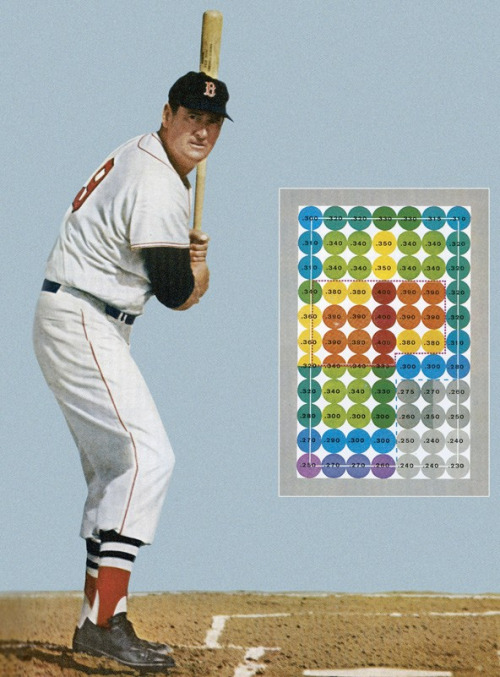
\includegraphics[scale=.35]{Images/Williams.jpg} 
      	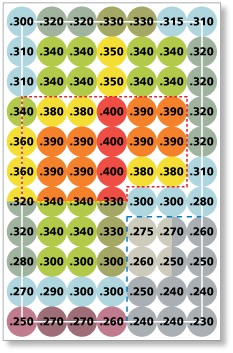
\includegraphics[scale=0.65]{Images/SZ.jpg}
      	\caption{Ted Williams carefully considered which pitch locations he preferred. In this image he divided the strike zone into pitch locations with specific probabilities of getting a hit. He labeled the baseballs with a personal batting average estimates for pitches in that location \citep{Williams1971}.}
      	\end{figure} 
The strike zone, enlarged on the right, contains baseballs labelled with the batting averages Williams estimated he achieved swinging at pitches in that location. Williams based his estimates on experience and intuition, because no such data existed. In fact, it took another 40 years for technology capable of collecting this type of data make it to MLB\textsuperscript{\textregistered}.

In 2008 MLB collaborated with a company called Sportsvision to implement a new technology called PITCHf/x\textsuperscript{\textregistered}, which collects the data necessary to analyze, visualize, and model William's location-based conception of hitting success.

\section{The Data} % ============================================
Sportvision, Inc., based in Chicago, provides the technology to collect PITCHf/x\textsuperscript{\textregistered} data. In 2008 Sportvision finished installing two high speed stereoscopic cameras in every MLB\textsuperscript{\textregistered} stadium. These cameras take 20 images of each pitch in flight and determine its path in three dimensions \citep{Fast2010}. Sportsvision licenses PITCHf/x\textsuperscript{\textregistered} data to Major League Baseball Advanced Media (MLBAM\textsuperscript{\textregistered}) \citep{Baumer2010}. 

        \begin{figure}[H]
      	\centering
      	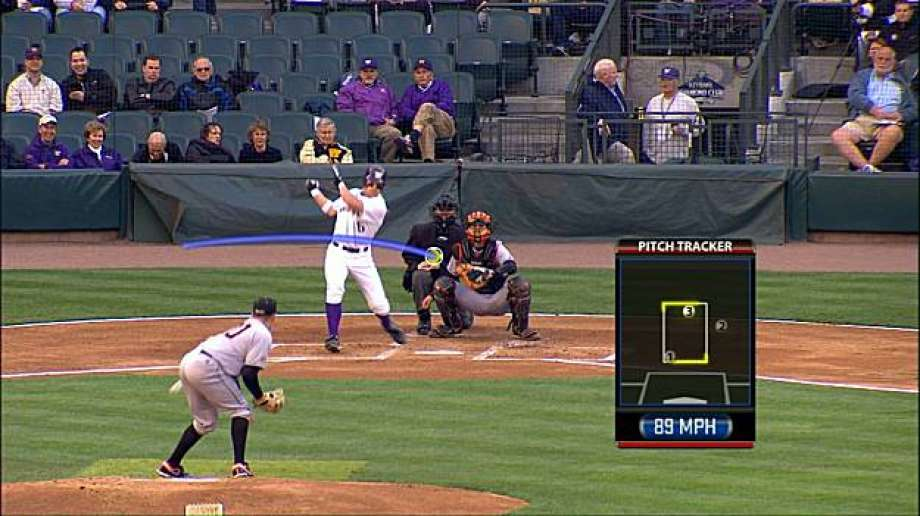
\includegraphics[scale=.4]{Images/PITCHfx.jpg} 
      	\caption{PITCHf/x\textsuperscript{\textregistered} data in your home. Television broacasts include pitch trajectory and strike zone data, in real time, for the viewer to see.}
      	\end{figure} 
MLBAM\textsuperscript{\textregistered} makes PITCHf/x\textsuperscript{\textregistered} data publicly available online in XML format, calling it ``Gameday'' data \citep{Sievert2014}. A homepage exists for every game, with links organizing data into XML tables with names such as {\it game, inning, at bat, pitch, team, player}, and {\it umpire} \citep{Sievert2014}. The {\it at bat} table, for example, contains data for 15 variables across 1,711,211 at bats. The format and size--on the order of gigabytes--of the data precludes direct download. Instead, XML scripts automate database ready downloads \citep{Adler2006}. We used a MySQL database, and \verb|dplyr| database management capabilities in R, to manipulate and store 13 PITCHf/x\textsuperscript{\textregistered} tables \citep{Tahaghoghi2006}, \citep{Wickham2016}. 

As an ``in-memory'' application, R uses a computer's limited RAM to host the R environment data \citep{Smith2013}. As a result, data manipulation on this scale requires ``memory management'' techniques \citep{Wickham2014}.  We applied Split-Apply-Combine operations to tables inside the MySQL database, before importing data frames to R \citep{Wickham2011}.

We collected the variables relevant for this research primarily from the {\it at bat} and {\it pitches} tables. We list these variables, with a short description, below \citep{Fast2007}.
  \begin{itemize}
  \item \verb|px| - location of the pitch on the horizontal axis when it passes through the strike zone (or the extended plane). \verb|px| is recorded in feet from the middle of home plate, from the catcher/umpire point of view.
  \item \verb|pz| - location of the pitch on the vertical axis when it passes through the strike zone plane, measured in feet above the ground. A negative value implies the ball bounced before reaching home plate
  \item \verb|des| - a short description of the outcome of the pitch, i.e. swing and miss, ground ball for out, ground ball for hit, etc.  
  \item \verb|id| - a unique id for a pitch within a game
  \item \verb|ab_id| - a unique id for each at bat  
  \item \verb|pitch_id| - a unique identification number for each pitch
  \item \verb|pitch_type| - a classification of the type of pitch, out of 18 possible types. For example, four seam fastball, two seam fastball, curveball, knuckle ball, etc.
  \item \verb|stand| - handedness of the batter; right or left.
  \item \verb|batter| - a unique ID for each hitter
  \end{itemize}

% Note the variable \verb|des|, short for `description,' that describes pitch outcomes. In this study, we use swing outcomes described in \verb|des| to define a Bernoulli random variable $S$ (Section 3.1) that equals one for a hit, and equals zero for {\it any} swing that does not result in a hit. This modifies the current standard, where analyses include only swings that end at bats \citep{Cross2015}, \citep{Baumer2010}, \citep{Fast2011}. We submit that {\it every} swing represents a trial, and failure to get a hit should be evaluated separately from the count in the at bat at the time of the trial.

Professional baseball teams, fans, and the baseball media (TV, radio, print, etc)  continually seek more insightful analysis. The collection and distribution of PITCHf/x\textsuperscript{\textregistered} data comes in response to this demand. In the next section we discuss the relevance of statistical analysis of baseball data, and of our research in particular, to these groups.

\section{Significance to Professional Baseball Organizations and Media}

Major League Baseball (MLB\textsuperscript{\textregistered}) teams exploy approximately 156 quantitative analysts, at a total cost of approximately \$15 million annually \citep{Lindbergh2016}. Teams strive to gain marginal competitive advantages; analysis of strike zone data provides just this sort of edge, so would generate interest. For example, exploratory data analysis indicate hitters have greater success in the lower one-third of the strike zone than in the top one-third; this contradicts baseball conventional wisdom, which advises pitchers to ``keep the ball down'' \citep{Stallings2003}. A model-based justification for this reversal would generate interest, because teams with this understanding could intelligently target and exploit the misconception. Taking it further, if these justifications are in biomechanical terms, biomechanists could analyze the relationship between body types and spatial success probabilities. MLB\textsuperscript{\textregistered} team scouting departments could use this information to more accurately predict hitting success for amateur players of varying builds, a notorously difficult but lucrative challenge. A second example at the player level, some MLB\textsuperscript{\textregistered} hitters, such as Joey Votto, have a keen interest in using the most sophisticated analytics available to understand the keys to their success and failure\citep{Daugherty2015}. The Votto model coefficient estimates could indicate imperceptible stregths and weaknesses to exploit or avoid. Votto, who carries a dog-eared copy of ``The Science of Hitting'' in his bag, pursues such nuances of his craft. 

With regard to baseball media interest, television broadcasts of MLB\textsuperscript{\textregistered} games, such as those on ESPN, TBS, or FOX regularly integrate PITCHf/x\textsuperscript{\textregistered}-based visuals into the viewing experience \citep{Cross2015}. 
        \begin{figure}[H]
      	\centering
      	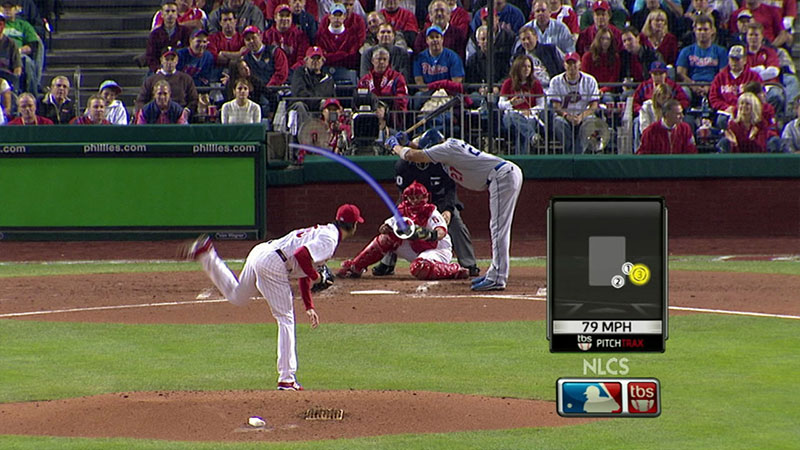
\includegraphics[scale=.4]{Images/PITCHfx2.jpg} 
      	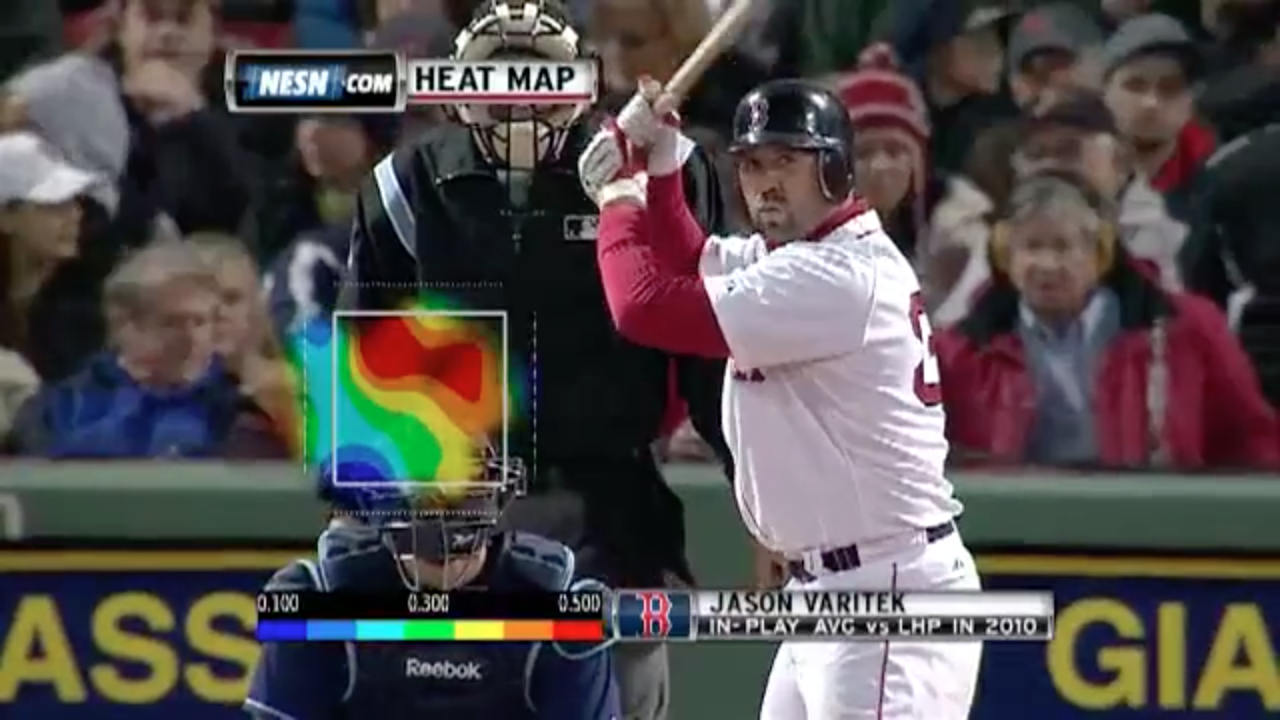
\includegraphics[scale=.25]{Images/Varitek.png} 
      	\caption{PITCHf/x\textsuperscript{\textregistered} data on TV. The top image shows pitch trajectory and strike zone location in a game on Turner Broacast System. The lower image includes what appears to be a smoothed empirical heat map on New England Sports Network. We envision an integration of these two visuals.}
      	\end{figure} 
Figure 1.3 shows two televised baseball features made possible by PITCHf/x\textsuperscript{\textregistered}; pitch trajectory and strike zone location; and a heat map. The heat map appears to be a smoothed empirical heat map. We envision more complete, modelled heat maps integrated with the strike zone location rectangle. Improved visuals serves the interests of MLB\textsuperscript{\textregistered} and the networks; ESPN\textsuperscript{\textregistered} and MLB\textsuperscript{\textregistered} recently agreed to an eight year, \$5.6 billion contract \citep{Newman2012}.

As the dollar amounts suggest, the pursuit of insightful analysis rages on. We are in a unique position, with the requisite expertise and data accessibility, to contribute such insightful analysis. In the next section we describe the preexisting statistical methods and research to provide context for this dissertation.

% spatial statistics \citep{Oliver2005}, and Bayesian hierarchical models \citep{Gelman2014}. We will employ these methodologies using the statistical software R \citep{R2015},baseball specific programming techniques \citep{Marchi2013}, 

\section{Context and Contributions}

% This research includes novel applications of advanced, cutting edge statistical techniques. In addition, as of publication, only one article in a peer reviewed journal focuses on our area of application. This combination---novel application of existing techniques to an unstudied area---constitutes a statistical research contribution. 

We analyze baseball data, but more specifically we analyze strike zone data. As of publication, \cite{Cross2015} constitutes the {\it only} statistical analysis of baseball data in a peer reviewed journal. This surprises, given the widespread enthusiam for baseball, until considering a few obstacles. First, PITCHf/x\textsuperscript{\textregistered} data collection began relatively recently, in 2008. Second, a potential analyst needs advanced skills in statistics, programming, and database management. The intersection of these analyst subsets proves quite small!  Third, MLB teams resist sharing. The teams conducting the most helpful research understandably prefer not to share it with other teams, and thereby dilute its value. In sum, these factors help explain the paucity of research. Howeer, our efforts rely on ample previous statistical research, and a some outside of statistics.

Our inspiration to model strike zone success owes Ted Williams a debt, for planting the initial seed with ``The Science of Hitting'' \citep{Williams1971}. As for an intersection of baseball and statistical research, \cite{Cross2015} provides the only peer reviewed literature to use as a starting point. The initial heat map in \cite{Cross2015} intimated--to us--that polar coordinates might facilitate explaining variation. 
        \begin{figure}[H]
      	\centering
      	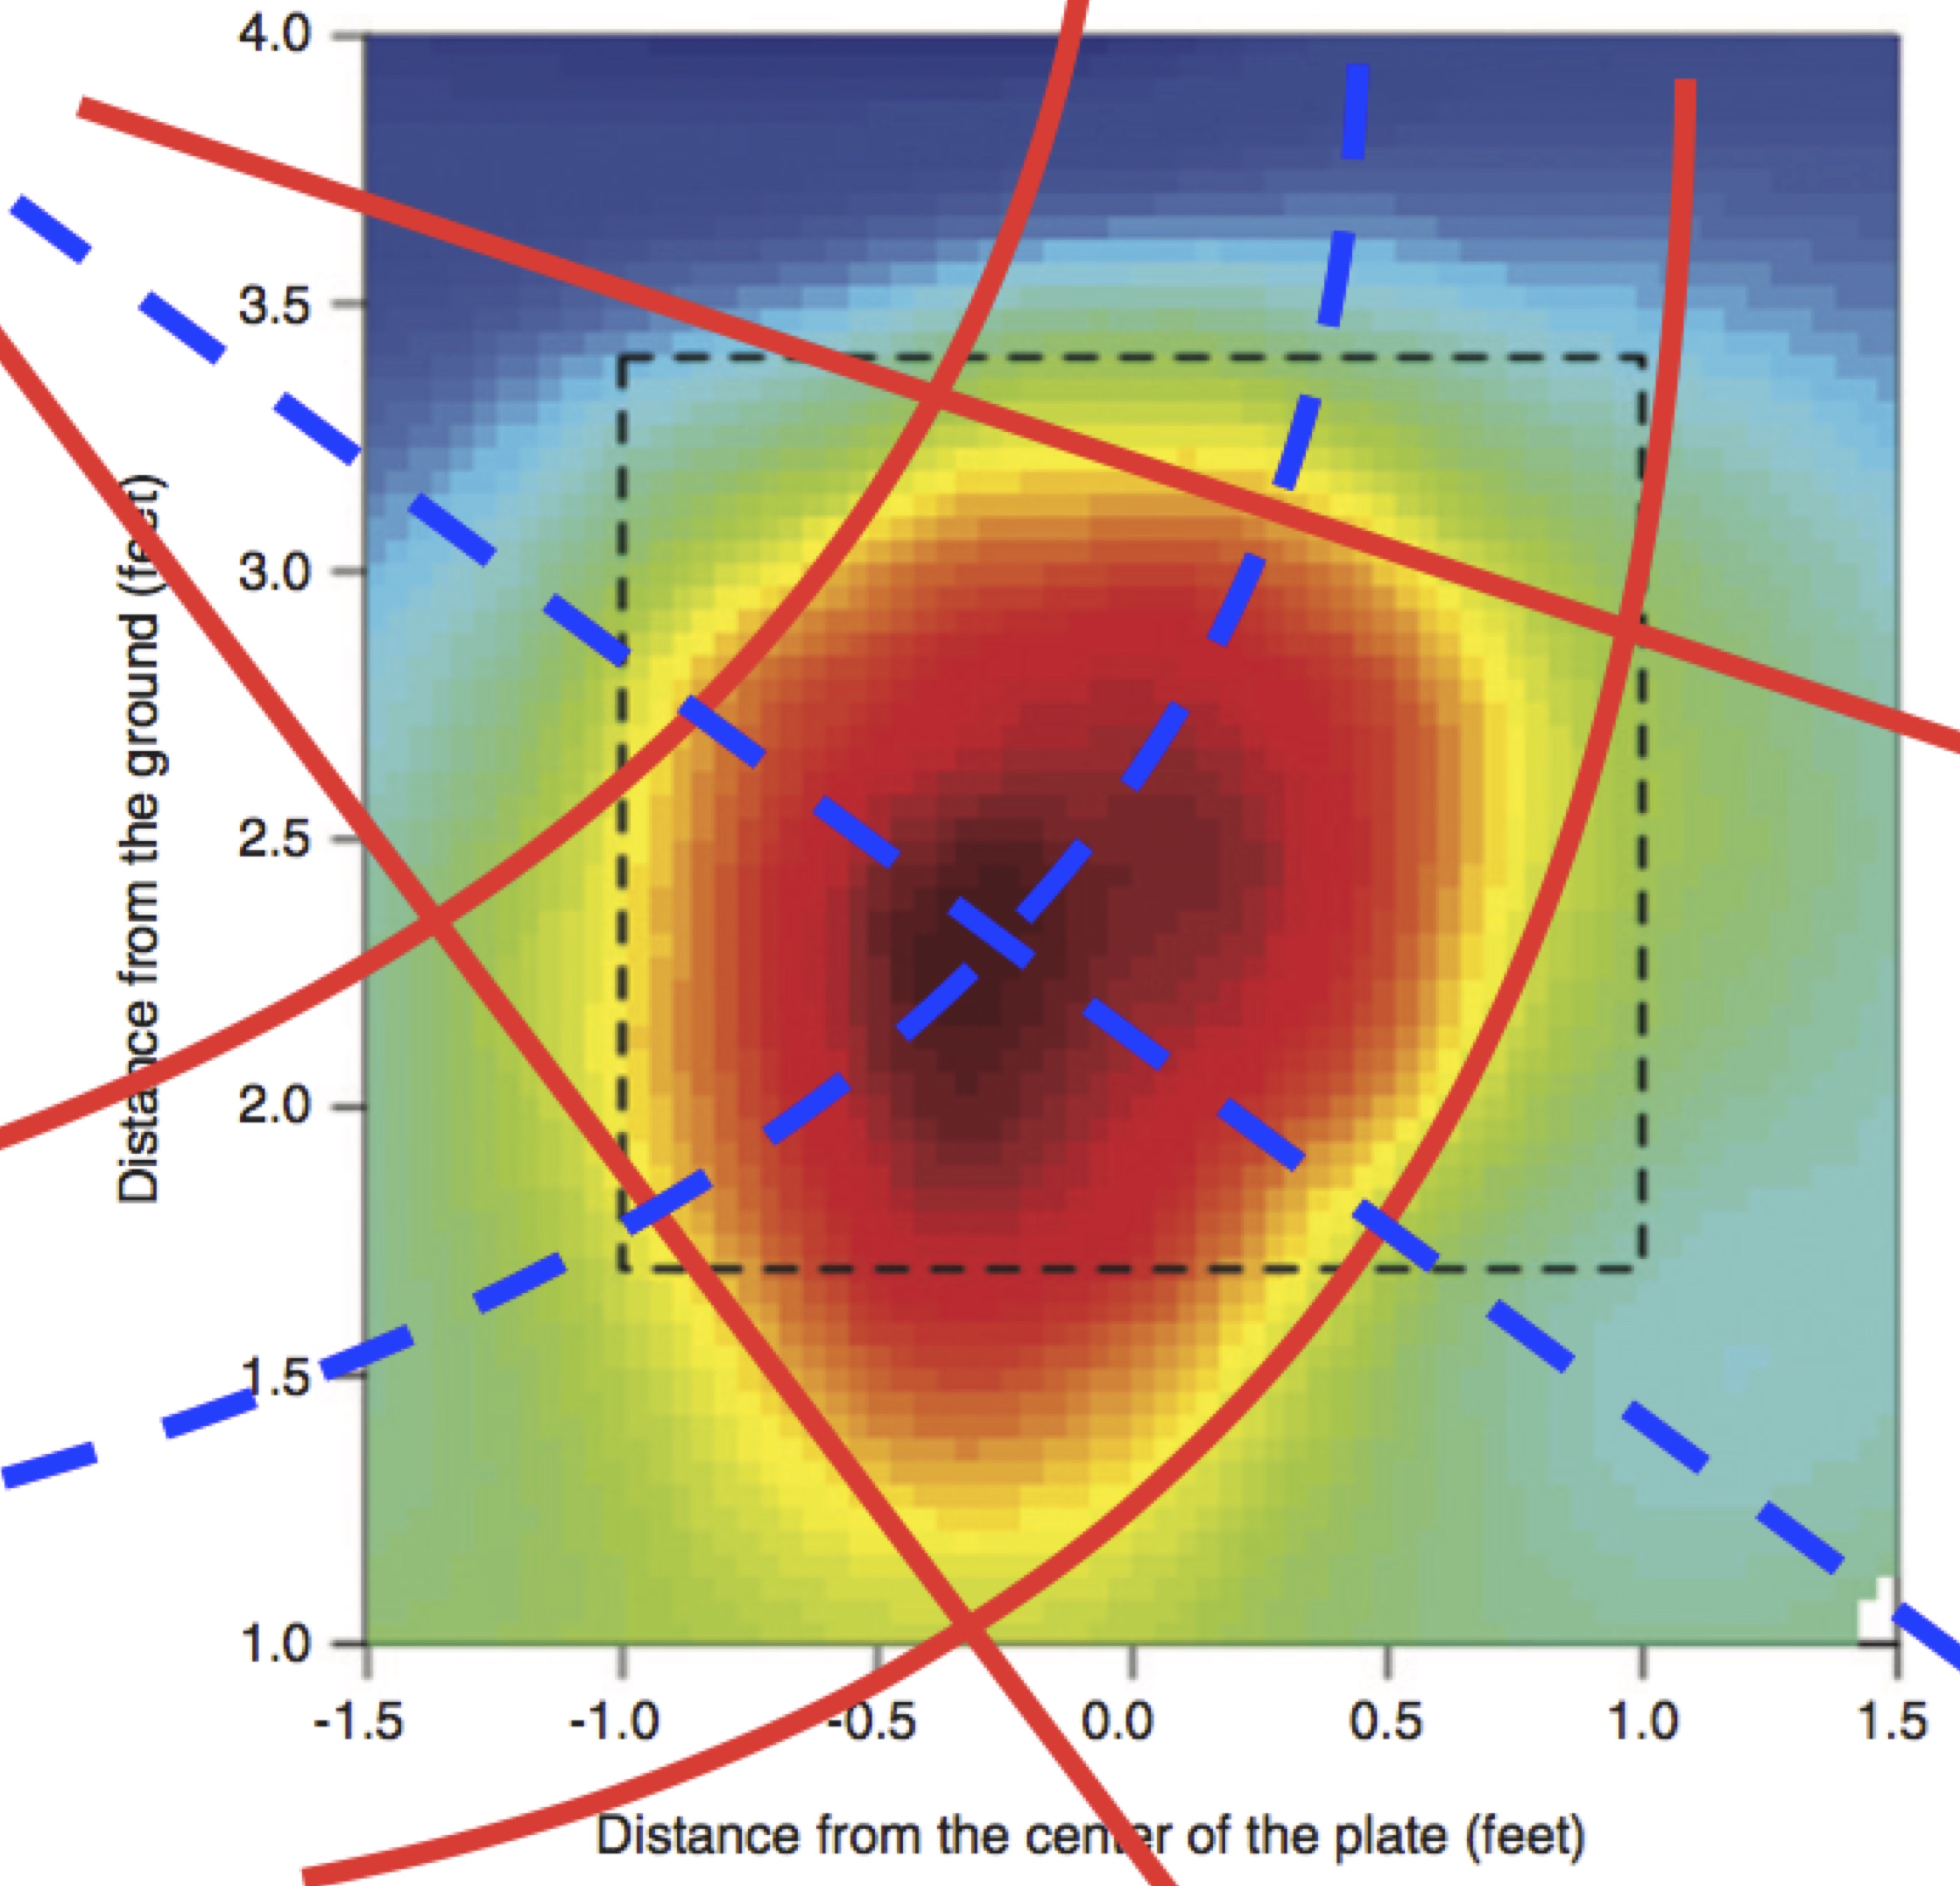
\includegraphics[scale=0.06]{Images/CrossPolar2.jpg} 
      	\caption{\cite{Cross2015} empirical heat map (undisclosed smoothing method), suggested polar coordinates. The added lines show our perception of polar coordinates.}
      	\end{figure}
The added lines in Figure 1.4 depict polar coordinates, albeit with a translated origin. This means concocting biomechanical covariates, from pitch locations in polar coordiates, involved choosing the polar origin. Glenn Fleisig at the American Sports Medical Institute \citep{Fleisig2002} and Brittany Dowling at Motus \citep{Dowling2016} provided feedback and encouragement in this effort. In contrast to \citep{Cross2015}, we sought a parametric model; Bernoulli response data suggests a generalized linear model (GLM), with logistic link \citep{Myers2012}. With a creative model in hand, early on \cite{Hosmer2013} provided a ``proof of concept'' test, essentially, for our polar-biomechanical model. From there, we followed two very distinct research paths: (i) improving heat map visualizations for our data and analysis, and by extension for all spatial data; and (ii) the "big N" problem for spatial random effects in a regression equation.

With regard to heat map innovations, empirical heat maps of our data provided the impetus for the first type of heat map innovation. Hadley Wickham's \verb|ggplot2|, with its ``layered grammar of graphics,'' supplied many of the necessary tools \citep{Wickham2009}, \citep{Wickham2010}. Doug Nychka's spatial data package \verb|fields| provided critical underlying spatial function in these efforts \citep{Nychka}. The second type of heat map innovation provides an improved method for presenting heat map confidence intervals. RStudio's ``interactive web application framework'' Shiny provided the dazzling new tools necessary for this innovation \citep{Shiny}.

Regarding the second path, generally speaking Bayesian hierarchical spatial models accomodate a spatial random effect handily \citep{Gelman2014}, \citep{Banerjee2014}, \citep{Oliver2005}. However, we fit our polar-biomechanical GLM to thousands, and tens of thousands of observations. This created big data challenges, including the "big N" problem. Hadley's \verb|dplyr| proved central to local database management \citep{Wickham2016}. The ``split-apply-combine strategy,'' in tandom with MySQL, provided important data wrangling tools \citep{Wickham2016}, \citep{Tahaghoghi2006}. After initial data wrangling steps, we took three swings at the ``big N'' problem: computational optimization, dimension reduction, and approximation.

We computationally optimized in the Bayesian programming language Stan, with the R interface \verb|rstan| \citep{rstan}, \citep{Gelman2015}. We pored over the manual \citep{STANtheMan}; and Stan developers Andrew Gelman, Rob Trangucci, and Bob Carpenter offered personal assistance \citep{Gelman}, \citep{Trangucci}, \citep{Carpenter}.

The second ``big N'' approach used tools developed by Andrew Finley, professor of Forrestry and Geography at Michigan State. Finley helped develop predictive process models, a dimension reduction technique and our second approach \citep{Banerjee2008}, \citep{Finley2012}. Predictive process models craftily reduce computational dimensionality, and we implemented this approach with Finley's package \verb|spBayes| \citep{Finley2013}.

Finally, we tried a cutting edge approximation techniques. The integrated nested laplace approximation (INLA), a mathematically complex and computationally sophisticated procedure, gives speedy estimates for models with a discrete domain \citep{Rue2009}, \citep{Rue2005}. Therefore, as best practices prescribe, we used a stochastic partial differential equation (SPDE) to modify our model domain to qualify for INLA \citep{Lindgren2011}, \citep{Lindstrom2016}. This exceedingly complex algorithm brings strengths and weaknesses \citep{Mondal2017}, \citep{Simpson2012b}, \citep{Rue2009}.

As this overview demonstrates, our research relied on the contributions of numerous other statisticians, programmers, scientists, and even a baseball player. Next, we lay out how this dissertation proceeds.

\section{Roadmap}

This dissertation has the following layout. In Chapter 2 we explore the problem of resolution selection for empirical heat maps, especially those with spatially varying data density. We present variable-resolution heat maps, a new option for addressing this problem. Two parts comprise Chapter 3. In the first part we create a generalized linear model for spatial hitter success probabilities, using biomechanical covariates. We manufacture these covariates by expressing pitch locations in the polar coordinate system and strategically translating the polar origin. In the second part, we explain the challenge of heat map confidence intervals, and describe the current, lacking best practices. Therefore, we present an interactive Shiny application solution \citep{Shiny}. In Chapter 4 we add a spatial random effect to the linear predictor in the polar-biomechanical GLM, and deal with the ``big N'' computational consequences. After defining the ``big N'' problem, and we explore three approaches to fitting a ``big N'' spatial generalized linear mixed model. 
